\documentclass[conference,compsoc]{IEEEtran}

	\ifCLASSOPTIONcompsoc
		\usepackage[nocompress]{cite}
	\else
		\usepackage{cite}
	\fi

	\usepackage[pdftex]{graphicx}
	\graphicspath{{./figuras/}}
	\DeclareGraphicsExtensions{.pdf,.jpeg,.png,.jpg}
	\usepackage{amsmath}
	\interdisplaylinepenalty=2500
	\usepackage{algorithmic}
	\usepackage{array}

	\ifCLASSOPTIONcompsoc
		\usepackage[caption=false,font=footnotesize,labelfont=sf,textfont=sf]{subfig}
	\else
		\usepackage[caption=false,font=footnotesize]{subfig}
	\fi

	\usepackage{fixltx2e}
	\usepackage{url}
	\hyphenation{re-a-li-za-ble sig-ni-fi-ca-do co-ne-xio-nes in-for-ma-cion}

	\def\abstractname{Resumen}
	\def\refname{Referencias}
	\def\figurename{Figura}
	\usepackage{SIunits}
	\usepackage{hyperref}

\begin{document}

	\title{Detector de nivel de agua y comunicaci\'on v\'ia ethernet con FPGA}

	\author{\IEEEauthorblockN{Marko Peshevski}
	\IEEEauthorblockA{Escola Polit\`ecnica Superior d'Enginyeria de Vilanova i la Geltr\'u\\
	Universitat Polit\`ecnica de Catalunya\\
	marko.peshevski@estudiant.upc.edu}}

	\maketitle

	\begin{abstract}

		En este trabajo se describe la implementaci\'on y utilizaci\'on de un sensor de nivel de agua
		econ\'omico sobre un n\'ucleo MicroBlaze en una placa de evaluaci\'on de la FPGA Spartan 6 de
		Xilinx. Para poder realizar la lectura de este sensor se utiliza un conversor anal\'ogico --
		digital de Microchip (MCP3002). Todo ello se muestra en una p\'agina web a trav\'es de un
		servidor que tambi\'en corre sobre el mismo n\'ucleo. La comunicaci\'on con la red se hace a
		trav\'es de Ethernet puesto que la placa de evaluaci\'on utilizada lo incorpora.

	\end{abstract}

	\section{Introducci\'on}

		En este trabajo se describe el desarrollo del software necesario sobre
		un n\'ucleo MicroBlaze de Xilinx para hacer la lectura de un sensor de
		nivel de agua de bajo coste y mostrar los datos en una p\'agina web que
		tambi\'en es servida por el mismo n\'ucleo. Para este prop\'osito se ha
		utilizado una placa de evaluaci\'on de la FPGA Spartan 6 de Xilinx
		(v\'ease Figura \ref{fig:fpga}). Esta placa en concreto es el modelo
		Spartan 6 LX9 MicroBoard de Avnet \cite{bib:avnet}.

		\begin{figure}[h!]
			\centering
			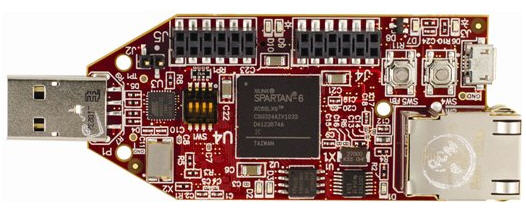
\includegraphics[width=0.35\textwidth]{./figuras/fpga.jpg}
			\caption{Placa de evaluaci\'on de la FPGA utilizada}
			\label{fig:fpga}
		\end{figure}

	\section{Objetivo}

		El principal objetivo de este trabajo es conseguir mostrar los datos le\'idos del conversor
		anal\'ogico -- digital en una p\'agina web accesible por cualquier navegador relativamente
		moderno\footnote{Que tenga soporte para WebSockets.}, y que esta visualizaci\'on tenga la
		menor latencia posible.

	\section{Sensor de nivel de agua}

		El sensor de nivel de agua utilizado en este trabajo es uno de muy bajo coste. En la Figura
		\ref{fig:sensor} se puede ver una imagen de este sensor. La placa de circuito impreso del sensor
		en cuesti\'on tiene un transistor NPN con su base conectada directamente a unas pistas en
		circuito abierto. Paralelas a las pistas en circuito abierto hay otras que est\'an conectadas a
		la tensi\'on de alimentaci\'on, a trav\'es de una resistencia limitadora de corriente de
		$100\,\ohm$. Cuando el agua entra en contacto con las pistas cierra el circuito, polarizando la
		base, y con ello amplificando la corriente de colector-emisor. Debido a que el sensor puede
		estar m\'as o menos hundido en agua, la longitud de pista hundida modificar\'a la resistencia
		que habr\'a en serie con la base del transistor. Variando esta resistencia se amplificar\'a en
		mayor o menor medida la corriente colector-emisor, y con ello se puede saber el nivel de agua
		del dep\'osito en el que estuviera hundido dicho sensor.

		\begin{figure}[h!]
			\centering
			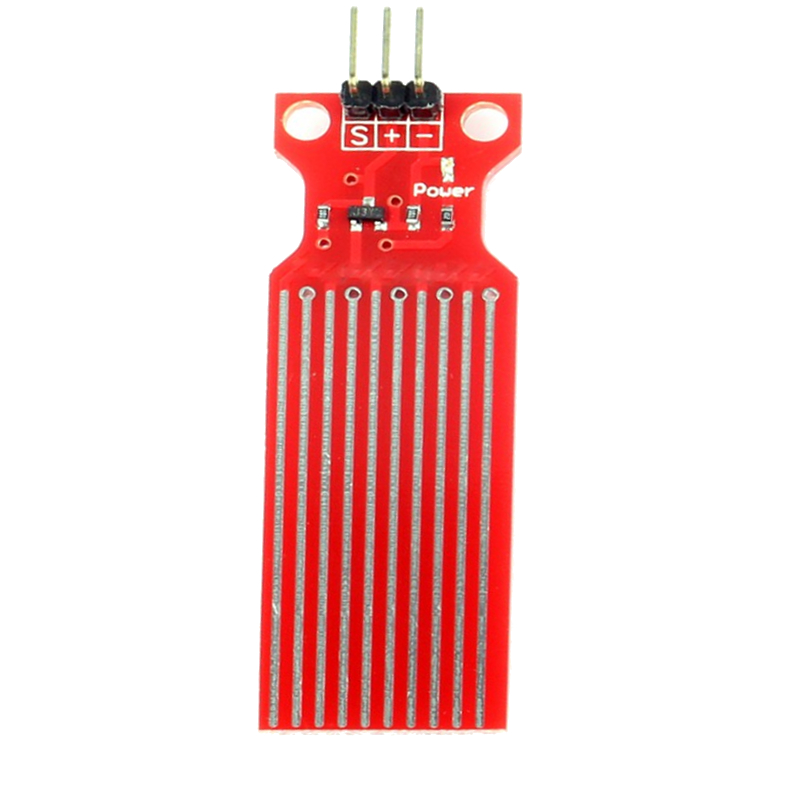
\includegraphics[width=0.2\textwidth]{./figuras/sensor.jpg}
			\caption{Sensor de nivel de agua utilizado para desarrollar este trabajo}
			\label{fig:sensor}
		\end{figure}

	\section{Conversor anal\'ogico -- digital}

		El conversor usado para leer el nivel de tensi\'on del sensor de nivel de agua es el conversor
		de 10 bits MCP3002 de Microchip\footnote{Se puede encontrar m\'as informaci\'on al respecto en:
		\url{http://www.microchip.com/wwwproducts/en/MCP3002}}. Este conversor se comunica con el
		n\'ucleo MicroBlaze a trav\'es de un canal serie SPI. Para obtener datos del mismo basta con una
		escritura de tan s\'olo 4 bits, a partir de los cuales el conversor ya responde con la medida de
		10 bits. \'Estos 4 bits, seg\'un el datasheet son:
		\begin{itemize}
			\item {Bit de start: inicio de comunicaci\'on, debe ser siempre de nivel alto;}
			\item {Bit SGL/DIFF: selecciona si se quiere utilizar el conversor para medidas pseudo-diferenciales o respecto al punto com\'un (masa);}
			\item {Bit ODD/SIGN: selecciona el orden de las entradas no inversora e inversora en el modo pseudo-diferencial, y cu\'al de los dos canales disponibles se quiere leer en el modo de medida respecto al punto com\'un;}
			\item {Bit MSBF: selecciona si se quiere recibir el bit m\'as significativo primero. Si este bit estuviera a nivel bajo el conversor primero devuelve los datos \emph{dos veces}, primero en orden decreciente (Most Significant Bit First) y luego en orden creciente (Least Significant Bit First).}
		\end{itemize}

		En la Figura \ref{fig:adc_spi} se puede ver resumido el protocolo que hace falta para
		comunicarse con el conversor.

		\begin{figure}[h!]
			\centering
			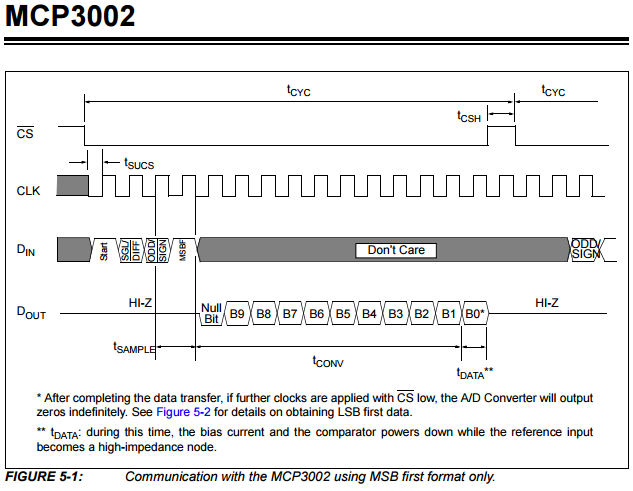
\includegraphics[width=0.49\textwidth]{./figuras/adc_spi.png}
			\caption{Resumen del protocolo SPI utilizado para leer del conversor anal\'ogico -- digital. Extra\'ida del datasheet del fabricante}
			\label{fig:adc_spi}
		\end{figure}

	\section{Interfaz Ethernet}

		Para desarrollar todo el apartado de comunicaci\'on v\'ia Ethernet y servidor web en este
		trabajo se ha partido de un ejemplo proporcionado por el fabricante de la placa de evaluaci\'on,
		Avnet \cite{bib:lwip-example}. En este ejemplo se utiliza la interfaz Ethernet a trav\'es de un
		n\'ucleo de propiedad intelectual (IP Core) de Xilinx llamado \emph{AXI\_Ethernetlite}. Este IP
		Core es el encargado de gestionar la comunicaci\'on a trav\'es de la interfaz ethernet, y desde
		el c\'odigo del n\'ucleo MicroBlaze se utiliza la misma desde un nivel relativamente alto. Este
		IP Core gestiona la pila de protocolo del modelo OSI hasta el nivel de enlace de datos (donde se
		hallan los protocolos de acceso al medio), siendo el resto de niveles (por encima del nivel de
		red, inclu\'ido), responsabilidad del usuario del IP Core.

	\section{Librer\'ia TCP/IP: lwIP}

		Para gestionar los niveles superiores del modelo OSI se utiliza la librer\'ia de protocolo
		TCP/IP llamada lwIP (lightweight IP). Esta es una librer\'ia de c\'odigo abierto
		especialmente dise\~nada para sistemas empotrados. Esta es la librer\'ia que, en el c\'odigo
		del n\'ucleo MicroBlaze, se encarga de gestionar las conexiones TCP, de comunicarse con el
		nodo lejano que intenta establecer una conexi\'on con el servidor, etc\'etera. Parte del
		c\'odigo del n\'ucleo que utiliza esta librer\'ia se reaprovecha del ejemplo del fabricante
		(\cite{bib:lwip-example}), aunque con modificaciones mayores para adaptarlo a la
		aplicaci\'on del trabajo.

	\section{WebSockets}

		Para conseguir el prop\'osito de m\'inima latencia posible en la visualizaci\'on de los datos en
		el navegador que accede a la p\'agina web servida por la FPGA se necesita comunicaci\'on
		bidireccional. Dicha comunicaci\'on no es f\'acilmente realizable con un servidor web de
		protocolo HTTP. Si se quisiera utilizar un protocolo HTTP para este f\'in lo que cabr\'ia hacer
		es que el cliente (navegador web) hiciera peticiones de tipo GET y POST para que el servidor le
		responda con los datos. Esto es tremendamente lento debido a que con el protocolo HTTP cada vez
		que se termina una petici\'on o respuesta a unos datos se cierra la conexi\'on. Una posible
		soluci\'on a este problema es utilizar WebSockets. Un WebSocket es, \emph{grosso modo}, una
		conexi\'on HTTP elevada a otro protocolo (WebSocket) que permite comunicaci\'on bidireccional en
		cualquier momento, sin que cliente o servidor tengan que hacer una petici\'on. Para el
		prop\'osito del trabajo esto es ideal puesto que una vez establecida la comunicaci\'on el
		servidor puede mandar informaci\'on al cliente tan a menudo como sea necesario. Se puede
		consultar toda la especificaci\'on del protocolo WebSockets en \cite{bib:ws}.

		En la Figura \ref{fig:ws_diagrama} se puede ver un diagrama resumiendo c\'omo funciona el
		protocolo WebSocket.

		\begin{figure}[h!]
			\centering
			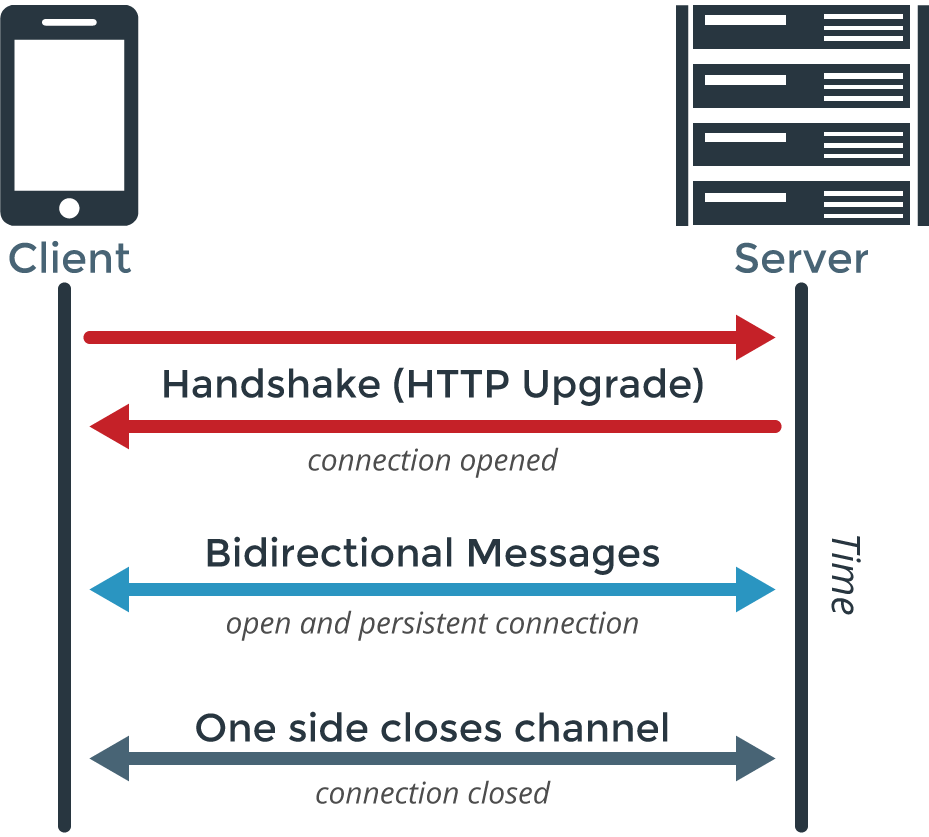
\includegraphics[width=0.3\textwidth]{./figuras/ws_diagrama.png}
			\caption{Diagrama resumen del protocolo WebSocket}
			\label{fig:ws_diagrama}
		\end{figure}

	\section{Lado cliente}

		Tras todo el resto la \'ultima parte que compone este trabajo es la visualizaci\'on de los
		datos en la p\'agina web. Para \'esta se ha utilizado un archivo HTML sencillo para crear un
		bot\'on que sirva para abrir la conexi\'on WebSocket (elevar el protoclo HTTP), y un
		gr\'afico utilizando librer\'ias de JavaScript ajenas \cite{bib:plotly-js}. En este
		gr\'afico se muestra directamente el valor de 10 bits $[0,1023]$ de salida del conversor
		anal\'ogico -- digital. Adem\'as de este gr\'afico (que s\'olo se dibuja una vez se tienen
		datos, es decir, una vez abierta la comunicaci\'on WebSocket), hace falta un peque\~no
		script en lenguaje JavaScript para gestionar la comunicaci\'on.

		\begin{figure}[h!]
			\centering
			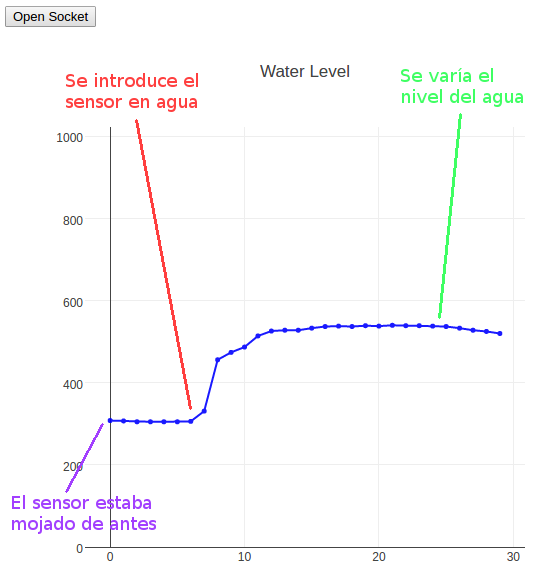
\includegraphics[width=0.49\textwidth]{./figuras/web_cliente.png}
			\caption{Web dise\~nada para este trabajo, mostrando brevemente el significado de los datos visualizados}
			\label{fig:web_cliente}
		\end{figure}

	% \section{Placa adaptadora}

	% 	Para facilitar las conexiones entre la placa FPGA y el sensor se ha dise\~nado una peque\~na
	% 	placa de circuito impreso. Esta placa tiene un z\'ocalo donde conectar el conversor
	% 	anal\'ogico -- digital y una tira de pines de conexi\'on para enchufarla a la placa de la
	% 	FPGA. Por otro lado tambi\'en tiene una tira de pines de conexi\'on para acoplar el sensor.

	\section{Conclusiones}

		Con el desarrollo descrito anteriormente se han conseguido los objetivos propuestos para
		este trabajo: mostrar el nivel de agua de un dep\'osito le\'ido con un sensor de muy bajo
		coste en una p\'agina web con la menor latencia posible, utilizando para ello un n\'ucleo
		MicroBlaze sobre una FPGA Spartan 6 de Xilinx.

	\section{Trabajo futuro}

		Por cuestiones l\'ogicas de tiempo y simplicidad, muchas cosas han quedado por desarrollar
		en este trabajo. Entre ellas, algunas de las m\'as relevantes ser\'ian:

		\begin{itemize}
			\item
			{

				Implementar el resto de funcionalidad del protocolo WebSocket: ser capaz de
				gestionar varias conexiones, abrir/cerrar conexiones, etc\'etera.

			}
			\item
			{

				Linealizar el sensor y calibrarlo de alguna manera. Puede ser necesario utilizar
				alg\'un amplificador del nivel de tensi\'on en la salida del sensor.

			}
			\item
			{

				Hacer que lo que se muestra en la web no sea solamente la lectura del conversor
				anal\'ogico -- digital sino algo con m\'as sentido.

			}
		\end{itemize}

	\bibliographystyle{IEEEtran}
	\begin{thebibliography}{1}

		\bibitem{bib:avnet}
			Xilinx Inc., \emph{Avnet Spartan-6 LX9 MicroBoard}, \url{https://www.xilinx.com/products/boards-and-kits/1-3i2dfk.html}.

		\bibitem{bib:lwip-example}
			Avnet Inc., \emph{LwIP Applications Software 201 for the Spartan-6 LX9 MicroBoard}, \url{https://forums.xilinx.com/xlnx/attachments/xlnx/EMBEDDED/9425/2/AvtS6LX9MicroBoard_SW201_lwIP_Apps_14_4_01.pdf}.

		\bibitem{bib:ws}
			I.~Fette y A.~Melnikov, \emph{The WebSocket Protocol}, \url{https://www.rfc-editor.org/rfc/rfc6455.txt}.

		\bibitem{bib:plotly-js}
			Plotly, \emph{What is plotly.js?}, \url{https://plot.ly/javascript/}.

		\bibitem{bib:repo}
			M.~Peshevski, \emph{SDAV\_mini-projecte}, repositorio Git con toda la informaci\'on sobre este trabajo, \url{https://github.com/markopesevski/SDAV_mini-projecte}.

	\end{thebibliography}

\end{document}




















%\begin{figure}[!t]
%\centering
%\includegraphics[width=2.5in]{myfigure}
% where an .eps filename suffix will be assumed under latex,
% and a .pdf suffix will be assumed for pdflatex; or what has been declared
% via \DeclareGraphicsExtensions.
%\caption{Simulation results for the network.}
%\label{fig_sim}
%\end{figure}

% An example of a double column floating figure using two subfigures.
% (The subfig.sty package must be loaded for this to work.)
% The subfigure \label commands are set within each subfloat command,
% and the \label for the overall figure must come after \caption.
% \hfil is used as a separator to get equal spacing.
% Watch out that the combined width of all the subfigures on a
% line do not exceed the text width or a line break will occur.
%
%\begin{figure*}[!t]
%\centering
%\subfloat[Case I]{\includegraphics[width=2.5in]{box}%
%\label{fig_first_case}}
%\hfil
%\subfloat[Case II]{\includegraphics[width=2.5in]{box}%
%\label{fig_second_case}}
%\caption{Simulation results for the network.}
%\label{fig_sim}
%\end{figure*}
%
% Note that often IEEE papers with subfigures do not employ subfigure
% captions (using the optional argument to \subfloat[]), but instead will
% reference/describe all of them (a), (b), etc., within the main caption.
% Be aware that for subfig.sty to generate the (a), (b), etc., subfigure
% labels, the optional argument to \subfloat must be present. If a
% subcaption is not desired, just leave its contents blank,
% e.g., \subfloat[].

% An example of a floating table. Note that, for IEEE style tables, the
% \caption command should come BEFORE the table and, given that table
% captions serve much like titles, are usually capitalized except for words
% such as a, an, and, as, at, but, by, for, in, nor, of, on, or, the, to
% and up, which are usually not capitalized unless they are the first or
% last word of the caption. Table text will default to \footnotesize as
% the IEEE normally uses this smaller font for tables.
% The \label must come after \caption as always.
%
%\begin{table}[!t]
%% increase table row spacing, adjust to taste
%\renewcommand{\arraystretch}{1.3}
% if using array.sty, it might be a good idea to tweak the value of
% \extrarowheight as needed to properly center the text within the cells
%\caption{An Example of a Table}
%\label{table_example}
%\centering
%% Some packages, such as MDW tools, offer better commands for making tables
%% than the plain LaTeX2e tabular which is used here.
%\begin{tabular}{|c||c|}
%\hline
%One & Two\\
%\hline
%Three & Four\\
%\hline
%\end{tabular}
%\end{table}

% Note that the IEEE does not put floats in the very first column
% - or typically anywhere on the first page for that matter. Also,
% in-text middle ("here") positioning is typically not used, but it
% is allowed and encouraged for Computer Society conferences (but
% not Computer Society journals). Most IEEE journals/conferences use
% top floats exclusively.
% Note that, LaTeX2e, unlike IEEE journals/conferences, places
% footnotes above bottom floats. This can be corrected via the
% \fnbelowfloat command of the stfloats package.
